\section{"4" Верификация преобразователя силы}

\begin{frame}[t]{Верификация преобразователя силы}
\framesubtitle{}
\begin{columns}[T,onlytextwidth]
\begin{column}{0.69\textwidth}
    \small
    \underline{Измерить характеристики} материала для случаев, когда \textbf{площадь приложения силы меньше}, чем \textbf{площадь активной части} сенсора.

    \textbf{Алгоритм}: 2 эксперимента: 
    
    1. Статический --- прикладывается статический груз с размером в сенсор для \underline{калибровки}.\\
    2. Динамический --- чувствительная область представляется в виде сетки $4\times4$. Происходит \textbf{касание} каждой \underline{области} \textbf{c одинаковым давлением}, но \underline{разной площадью контакта}.

    \textbf{Входные данные}: показания разработанного датчика и значение реально приложенной нагрузки.

    \textbf{Выходные данные}: разница между нормализованным значением с датчика и реальной нагрузкой.

    \textbf{Допустимая ошибка}: 10\%

    \textbf{Предположения}: 1) материал обладает вязко-эластичными свойствами, поэтому надо учитывать гистерезис.
\end{column}
\begin{column}{0.29\textwidth}
    \vspace{-1.0cm}
\begin{figure}[H]
\begin{subfigure}{0.99\textwidth}
        \centering
        \centering\includegraphics[height=3cm,width=1\textwidth,keepaspectratio,page=5]{./tikz_pictures.pdf}
        \caption*{Поверхность \\ как $4\times4$ сетка}
\end{subfigure}

\begin{subfigure}{0.99\textwidth}
    \centering\includegraphics[height=3cm,width=1\textwidth,keepaspectratio,page=4]{./tikz_pictures.pdf}
    \caption*{Все насадки}
\end{subfigure}

\end{figure}
\end{column}
\end{columns}
\end{frame}

\note{\small \setlength{\parindent}{20pt}

Решив задачу номер 3, то есть имея конструкцию ноги, возможно разработать сенсор, подходящий для конкретной области применения. Как было сказано ранее, необходимо измерить характеристики материала для случаев когда площадь приложения силы меньше, чем площадь активной части сенсора.

Для этого было разработано 2 эксперимента. Первый, статический, где на объект прикладывался статический груз с размером сенсора, нужен для калибровки. Таким образом я считал, что все сенсоры работают единообразно.

Второй, динамический, основной. Для этого сенсор представлялся в виде сетки 4х4, на картинке *тык*. С помощью эталонного датчика силы, на который была прикреплена насадка *тык*, обеспечивающую конкретную площадь контакта, проводилась касание каждой области сетки. 

После эксперимента, нормализовались значения между эталонным датчиком (его значения принимались за 1), и откалиброванным исследуемым датчиком. Смотрелась разница. 

Допустимой ошибкой я посчитал 10 процентов, такая ошибка принята в физических экспериментах.
}

\begin{frame}[t]{Статический эксперимент}
    \begin{columns}[T,onlytextwidth]
        \begin{column}{0.52\textwidth}
            \begin{eqnarray}
                V_{out} = V_0 + p[k_p + k_e(1-e^\frac{-(t-t_0)}{\tau_{res}})](1-e^{-\frac{A}{p}}) \\
                k_p = A_1e^{-A_2p} \\ \tau_{res} = B_0 + B_1e^{-\frac{p}{B_2}}
            \end{eqnarray}
            Где $V_0$ -- начальное напряжение, \\ $p$ -- приложенное давление, \\ $A_i,\ B_i,\ \tau_{res},\ k_i$ искомые параметры, \\  $t$ -- текущее время, $t_0$ -- время начала нажатия.
            % \\ \alert{Апробированна модель для калибровки датчика}
        \end{column}
        \begin{column}{0.45\textwidth}
            \vspace{-0.5cm}
            \begin{figure}[H]
                \begin{subfigure}{0.99\textwidth}
                    \centering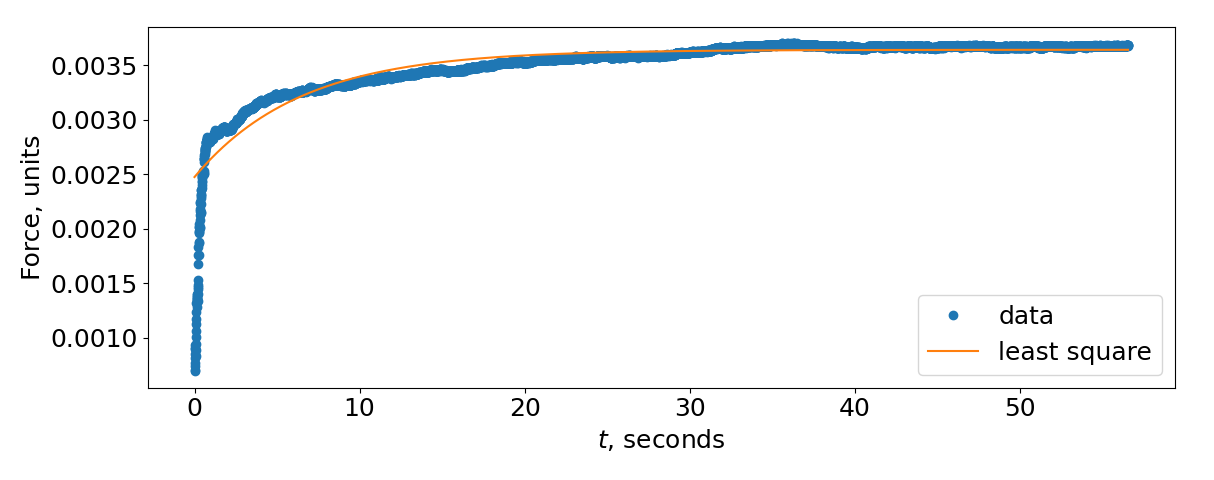
\includegraphics[height=2.8cm,width=1\textwidth,keepaspectratio]{least_square_model.png}
                    \caption*{График регрессии}
                \end{subfigure}

                \vspace{-0.3cm}
                \begin{subfigure}{0.99\textwidth}
                    \centering
                    \centering\includegraphics[height=3.4cm,width=1\textwidth,keepaspectratio,page=6]{./tikz_pictures.pdf}
                    \caption*{Экспериментальная установка}
                \end{subfigure}
            \end{figure}
        \end{column}
    \end{columns}
\end{frame}

\note{\small \setlength{\parindent}{20pt}

Статический эксперимент. Для калибровки использовался робастный метод наименьших квадратов, экспериментальная установка справа *тык*, формула для регрессии --- слева *тык*. Она основана на знании того, что у нас вязко-эластичный материал, обладающий гистерезисом. Поэтому необходимо учитывать время контакта с поверхностью.

Экспериментальная установка показана ниже *тык*.

Как можно заметить по графику справа, эта формула подходит для калибровки.}

\begin{frame}[t]{Динамический эксперимент: Установка}
    \vspace{0.2cm}
    \centering\includegraphics[height=6.5cm,width=1\textwidth,keepaspectratio,page=7]{./tikz_pictures.pdf}
\end{frame}

\note{\small \setlength{\parindent}{20pt}

Так как динамический эксперимент требует многократное повторение действий, где важна точность силы нажатия, то было решено создать автоматизированную робототехническую установку *тык*. 

Минимизация ошибки по установке манипулятора была реализована с помощью технического зрения.

Манипулятор необходим, так данная установка позволяет проводить не только контактные эксперименты, но также и прокатывать вали по сенсору, что ближе к кинематике движения робота. Более того, мы можем проверять и калибровать сенсор уже установленный на ногу робота.
}

\begin{frame}[t]{Результаты динамического эксперимента}
    \begin{figure}[H]
        \begin{subfigure}{0.49\textwidth}
            \centering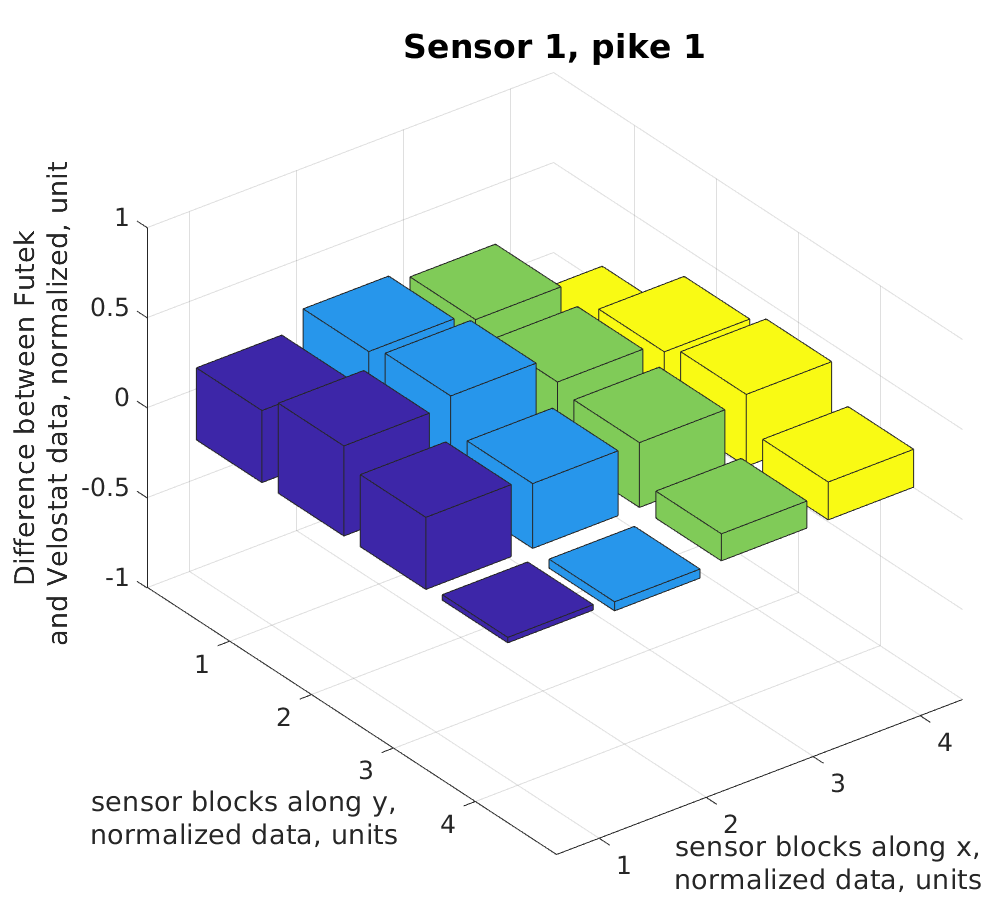
\includegraphics[height=5cm,width=1\textwidth,keepaspectratio]{sens1_pike1.png}
            \caption*{2 мм диаметр насадки}
        \end{subfigure}
        \begin{subfigure}{0.49\textwidth}
            \centering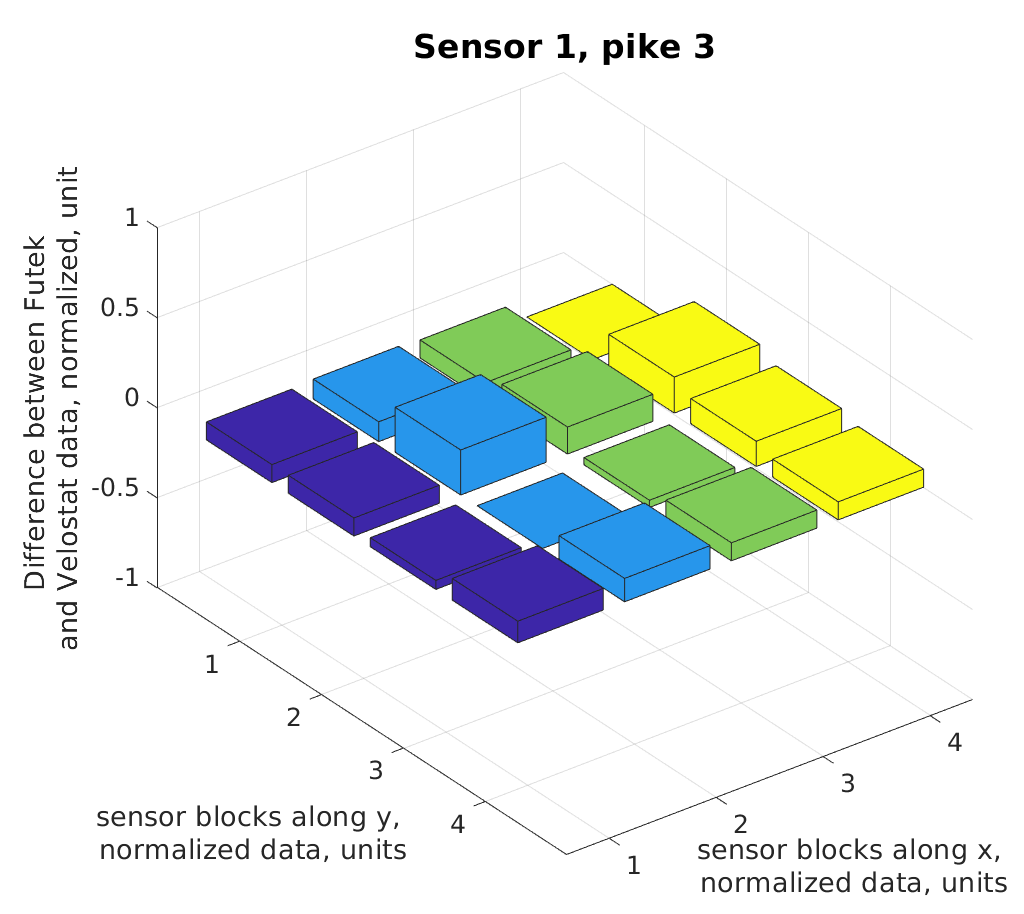
\includegraphics[height=5cm,width=1\textwidth,keepaspectratio]{sens1_pike3.png}
            \caption*{8 мм диаметр насадки}
        \end{subfigure}
    \end{figure}
    \vspace{-0.8cm}
    \alert{Одинаковые данные, когда площадь нажатия превышает 25\% от площади датчика}
\end{frame}

\note{\small \setlength{\parindent}{20pt}

Результатом изысканий получилось, что можно использовать сенсор, когда площадь нажатия превышает 25 площади датчика.

На слайде можно увидеть 3д гистограмму *тык*, где представлена нормализованная разница между эталонным датчиком и исследуемым для каждого сегмента датчика. Слева при использования насадки в 2 мм диаметром, а справа при 8 мм.
}